
%%%%%%%%%%%%%%%%%%%%%%% file typeinst.tex %%%%%%%%%%%%%%%%%%%%%%%%%
%
% This is the LaTeX source for the instructions to authors using
% the LaTeX document class 'llncs.cls' for contributions to
% the Lecture Notes in Computer Sciences series.
% http://www.springer.com/lncs       Springer Heidelberg 2006/05/04
%
% It may be used as a template for your own input - copy it
% to a new file with a new name and use it as the basis
% for your article.
%
% NB: the document class 'llncs' has its own and detailed documentation, see
% ftp://ftp.springer.de/data/pubftp/pub/tex/latex/llncs/latex2e/llncsdoc.pdf
%
%%%%%%%%%%%%%%%%%%%%%%%%%%%%%%%%%%%%%%%%%%%%%%%%%%%%%%%%%%%%%%%%%%%


\documentclass[runningheads,a4paper]{llncs}
\usepackage{amssymb,amsmath}
\setcounter{tocdepth}{3}
\usepackage{graphicx}
\usepackage{enumitem}
\usepackage{url}

%\usepackage[T2A]{fontenc}
%\usepackage[utf8x]{inputenc}
%\usepackage[russian,english]{babel}



\begin{document}

\mainmatter  % start of an individual contribution

% first the title is needed
\title{Parallel Multipoint Approximation Method for Large Scale Optimization Problems 
\thanks{This study was supported by the Russian Science Foundation, project No. 16-11-10150.}}

% a short form should be given in case it is too long for the running head
\titlerunning{Parallel Multipoint Approximation Method}

\author{ Victor P. Gergel%(ORCID 0000-0002-4013-2329)
$^1$ \and
Konstantin A. Barkalov%(ORCID 0000-0001-5273-2471)
$^1$ \and
Evgeny A. Kozinov%(ORCID 0000-0001-6776-0096)
$^1$ \and
Vassili V. Toropov%(ORCID 0000-0002-7017-5055)
$^{1,2}$
}
%
\authorrunning{V.P. Gergel \and K.A. Barkalov \and E.A.Kozinov \and V.V. Toropov}
% (feature abused for this document to repeat the title also on left hand pages)

% the affiliations are given next; don't give your e-mail address
% unless you accept that it will be published
\institute{$^1$Lobachevsky State University of Nizhny Novgorod, Nizhny Novgorod, Russia\\
\email{\{victor.gergel, konstantin.barkalov, evgeny.kozinov\}@itmm.unn.ru}\\
$^2$Queen Mary University of London, London, UK\\
\email{v.v.toropov@qmul.ac.uk}\\
}

%
% NB: a more complex sample for affiliations and the mapping to the
% corresponding authors can be found in the file "llncs.dem''
% (search for the string "\mainmatter" where a contribution starts).
% "llncs.dem" accompanies the document class "llncs.cls".
%

%\toctitle{Lecture Notes in Computer Science}
%\tocauthor{Authors' Instructions}
\maketitle

\begin{abstract}
The paper presents a new development in the Multipoint Approximation Method (MAM) that makes it capable of handling large scale problems. The approach relies on approximations built in the space of design variables within the iterative trust-region-based framework of MAM. 
With the purpose of solving the problems of high dimensionality in a reasonable time, a parallel variant of the Multipoint Approximation Method (PMAM) has been developed. It was supposed that the values of the objective function and of the constraints were computed using the distributed memory (on several cluster nodes), whereas the optimization module run on a single node using the shared memory. The numerical experiments have been carried out on a benchmark example of structural optimization.

\keywords{design optimization, multidisciplinary optimization, multipoint approximation method, parallel computing.}
\end{abstract}

\section{Introduction}

In the present paper, the multipoint approximation method (MAM \cite{Toropov1989,Toropov1992,ToropovFilatov1993}) and its application to the large scale optimization problems are considered. In problems with a large (in the order of hundreds) number of design variables MAM proved to be efficient, e.g. in turbomachinery applications \cite{ShahparPolynkinToropov2008,PolynkinToropovShahpar2008,PolynkinToropovShahpar2010}. This method is an iterative optimization technique based on mid-range approximations built in trust regions. A trust region is a sub-domain of the design space in which a set of design points, produced according to a small-scale design of experiments (DoE), are evaluated. These and a subset of previously evaluated design points are used to build metamodels of the objective and constraint functions that are considered to be valid within a current trust region. The trust region will then translate and change size as optimization progresses. The trust region strategy has gone through several stages of development to account for the presence of numerical noise in the response function values \cite{KeulenToropovMarkine1996,ToropovKeulenMarkine1996} and occasional simulation failures \cite{ToropovMarkineHolden1999}. The mid-range approximations used in the trust regions, as originally suggested in \cite{Toropov1989} for structural optimization problems, are intrinsically linear functions (i.e. nonlinear functions that can be led to a linear form by a simple transformation) for individual sub-structures, and assembly of them for the whole structure. This was enhanced by the use of gradient-assisted metamodels \cite{ToropovFilatov1993}, use of simplified numerical models that is also termed a multi-fidelity approach,\cite{ToropovMarkine1996} and the use of analytical models derived by Genetic Programming \cite{ToropovAlvarez1998}. One of the recent developments \cite{PolynkinToropov2012} involved the use of approximation assemblies, i.e. a two stage approximation building process that is conceptually similar to the original one used in \cite{Toropov1989} but is free from the limitation that lower level approximations are linked to individual substructures.

The Moving Least Squares Method (MLSM) was proposed in \cite{LancasterSalkauskas1981} for smoothing and interpolation of scattered data and later used in the mesh-free form of the FEM \cite{Liszka1984}. As suggested in \cite{ChoiYounYang2001}, it can be used as a technique for metamodelling and used in MDO frameworks. The MLSM is a weighted least squares method where the weights depend on the Euclidean distance from a sample point to where the surrogate model is to be evaluated. The weight value for a certain sample point decays as the distance increases. Describing the weight decay with a Gaussian function tends to be the most useful option even though many others have been evaluated in \cite{ToropovSchrammSahaiJones2005}. As demonstrated in \cite{PolynkinToropov2010}, the cross-validated MLSM can be used both for design variable screening and for surrogate modelling. In order to create an efficient MDO framework for problems with disparate discipline attributes \cite{OllarToropovJones2014} extended the optimization approach of MAM to the use of local DOEs and MLS approximations built in different subspaces of the total design variable space corresponding to the individual disciplines. The subspaces are finally combined into the total design variable space in which the resulting MDO problem is solved.

This paper presents a Parallel Multipoint Approximation Method that makes it capable of handling problems with the number of design variables in the order of thousands. The parallel variant of the algorithm (with the use of the shared memory) has been developed with the purpose of minimizing the worktime of the part of the algorithm related to constructing the approximation and solving the approximated problem and not related to computing the values of the objective function and  constraints. The processes of computing the values of the objective function and constraints (with the use of the 
distributed memory) are supposed to be parallelized already.

\section{The Multipoint Approximation Method}
\label{sec:MAM}

It is useful to start with a brief description of MAM. A typical formulation of a constrained optimization problem that MAM works with is as follows:
\begin{equation}
  \label{eq:problem}
  \begin{array}{c}
  \min\limits_{a_i \le x_i \le b_i}F_0(x) \\
  s.t.\; F_j(x) \le 1,\; j=1,\dots ,M,
  \end{array}
\end{equation}
where $x$ is the vector of design variables, $a$ and $b$ are the lower and upper bounds for the design variables, respectively, $F_0(x)$ is the objective function, and $F_j(x)$ are the constraints. The numbers of design variables and constraints are $n$ and $M$, respectively. MAM attempts to solve this problem by using approximations of the objective function and constraints in a series of trust regions. The trust region strategy seeks to zoom in on the region where the constrained minimum is achieved. It aims at finding a trust region that is sufficiently small for the approximations to be of sufficiently good quality to improve the design, and that contains the point of the constrained minimum as its interior point. The main loop of the MAM is organized as follows.
\\

\textbf{Algorithm (MAM).}
\begin{enumerate}
\item Initialization: choose a starting point $ x^0$ and initial trust region $[ a^0,  b^0]$ such that $ x^0 \in [ a^0,  b^0]$.
\item At the $k$-th iteration the current approximation to the constrained minimum is $ x^k$, the current trust region is $[ a^k,  b^k] \subset [ a^0,  b^0]$.
  \begin{enumerate}[label=(\alph*)]
    \item Design of Experiments (DoE): a set of points $ x_k^i \in [ a^k,  b^k]$ is chosen to be used for approximation building. Responses are evaluated at the DoE points and approximations are built using the obtained values. Currently, the pool of approximation methods available in MAM consists of a metamodel assemblies \cite{PolynkinToropov2012} and the moving least-squares metamodels \cite{LancasterSalkauskas1981,Liszka1984,ChoiYounYang2001,ToropovSchrammSahaiJones2005}. Other metamodel types could be used as well.

    Denote the approximate objective function and constraints by $\widetilde{F}^k_0(x)$ and $\widetilde{F}^k_j(x)$, respectively.
    \item The original optimization problem (\ref{eq:problem}) is replaced by the following problem:
    \begin{equation}
      \label{eq:problem_approx}
      \begin{array}{c}
      \min\limits_{a_i^k \le x_i ^k\le b_i}\widetilde{F}^k_0(x) \\
      s.t.\; \widetilde{F}^k_j( x) \le 1,\; j=1,\dots ,M,
      \end{array}
    \end{equation}
    The approximate problem (\ref{eq:problem_approx}) is solved using Sequential Quadratic Programming (SQP) and the solution of this problem determines the center of the next trust region.
    \item The size of the next trust region is determined depending on the quality of approximations at the previous iteration, on the history of the points $ x^k$, and on the size of the current trust region \cite{KeulenToropovMarkine1996}.
    \item The termination criterion is checked (it is a part of the trust region strategy and depends on the position of the point $ x^{k+1}$ in the current trust region, the size of the current trust region and the quality of approximations). If the termination criterion is satisfied, the algorithm proceeds to step 3. Otherwise, it returns to step 2.
  \end{enumerate}
  \item Optimization terminates. The obtained approximation to the solution of the problem (\ref{eq:problem}) is $ x^{k+1}$.
\end{enumerate}

The selection of the approximations $\widetilde{F}^k_j(x),\; j=0, \dots ,M,$ is such that their evaluation is inexpensive as compared to the evaluation of the original response functions $F_j(x)$. For example, intrinsically linear functions were successfully used for a variety of design optimization problems in the works \cite{ToropovFilatov1993,KeulenToropov1997}. The approximations are determined by means of the weighted least squares:
\begin{equation}\label{eq:least_sq}
\min \sum_{p=1}^P{w_{pj}\left[ F_j(x_p)- \widetilde{F}^k_j(x_p,a_j) \right]^2}.
\end{equation}
In (\ref{eq:least_sq}) minimization is carried out with respect to the tuning parameters $a_j$; $w_{pj}$ are the weight coefficients, and $P$ is the number of sampling points in Design of Experiments (DoE) which must not be less than the number of parameters in the vector $a_j$.

The weight coefficients $w_{pj}$ strongly influence the difference in the quality of the approximations in different regions of the design variable space. Since in realistic constrained optimization problems the optimum point usually belongs to the boundary of the feasible region, the approximation functions should be more accurate in such domain. Thus, the information at the points located near the boundary of the feasible region is to be treated with greater weights. In a similar manner a larger weight can be allocated to a design with a better objective function, see \cite{ToropovFilatov1993,KeulenToropov1997}.

As optimization steps are carried out, a database with response function values becomes available. In order to achieve good quality approximations in the current trust region, an appropriate selection of DoE points must be made. In this work, DoE points in each trust region is generated randomly. Generally, points located far from the current trust region would not contribute to the improvement of the quality of the resulting approximations in the trust region. For this reason only points located in the neighborhood of the current trust region are taken into account, as depicted in Fig.~\ref{fig:trustregion}.
\begin{figure}[ht]
    \centering
    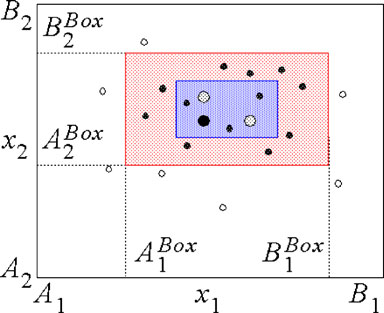
\includegraphics[width=0.5\textwidth]{trustregion.png}
    \caption{Current trust region (smaller box) and its extension (larger box): points outside the larger box are not used for building the approximate functions}
    \label{fig:trustregion}
\end{figure}
A box in the space of design variables, which is approximately 1.5 to 1.8 times larger than the box representing the current trust region, was found by numerical experimentation to be a reasonable choice for the size of the neighborhood.

In this work an approach is used that is based on the assembly of different approximate models $\{\varphi_l\}$ into one metamodel using the following form (note that the indices $j$ and $k$ are suppressed to simplify notation):
\begin{equation}\label{eq:assembly}
\widetilde{F}(x) = \sum_{l=1}^{NF}{b_l\varphi_l(x)},
\end{equation}
where $NF$ is the number of regressors in the model pool $\{\varphi_l\}$ and $b_l$ are corresponding regression coefficients.
The used procedure consists of two subsequent steps. In the first step, the parameters $a_l$ of individual functions (regressors) $\varphi_l$ in (\ref{eq:assembly}) are determined by solving a weighted least squares problem using a specified a DoE of $P$ points:
%\begin{equation}\label{eq:least_sq}
\[
\min \sum_{p=1}^P{w_{p}\left[ F(x_p)- \varphi_l(x_p,a_l) \right]^2},
\]
%\end{equation}
where minimization is carried out with respect to the tuning parameters $a_l$.

In the second step, based on the same DoE and keeping the obtained parameters $a_l$ fixed, a vector $b$ in (\ref{eq:assembly}) is estimated using the following formulation
\[
\min \sum_{p=1}^P{w_{p}\left[ F(x_p)- \widetilde{F}(x_p,b) \right]^2},
\]
that leads to solving a linear system of $NF$ equations with $NF$ unknowns $b_l$, where $NF$ is the number of regressors in the model pool $\{\varphi_l\}$.

The selection of the regressors $\{\varphi_l\}$ is based on the number of sampling points currently located in the trust region. In the mid-range approximation framework, inexpensive approximate models for objective and constraint functions are built using minimum required number of sampling points. The simplest case is a linear function of the tuning parameters $a$:
\[
\varphi(x) = a_0 + \sum_{i=1}^N{a_i x_i}.
\]

This structure can be extended to an \textit{intrinsically linear} function. Such functions are nonlinear, but they can be led to linear ones by simple transformations. The most useful function among them is the multiplicative function
\[
\varphi(x) = a_0 \prod_{i=1}^N{x{_i}^{a_i}}.
\]

Intrinsically linear functions have been successfully used for a variety of design optimization problems. 
The advantage of these approximation functions is that a relatively small number $N+1$ ($N$ is number of design variables) of tuning parameters $a_i$ is to be determined, and the corresponding least squares problem is solved easily. This is the most important feature of such approximations as it allows applying them to large scale optimization problems.

Other intrinsically linear functions may be considered in the model pool, e.g.
\[
\varphi(x) = a_0 + \sum_{i=1}^N{a_i/x_i},
\]
\[
\varphi(x) = a_0 + \sum_{i=1}^N{a_i x_i^2},
\]
\[
\varphi(x) = a_0 + \sum_{i=1}^N{a_i/x_i^2},
\]
\[
\varphi(x) = a_0 + \sum_{i=1}^N{a_i x_i^3},
\]
\[
\varphi(x) = a_0 + \sum_{i=1}^N{a_i/x_i^3}.
\]

As more points are added to the database the approximations may be switched to higher quality models, e.g. a rational model
\begin{equation}\label{eq:rational}
\varphi(x) = \frac{a_1 + a_2x_1 + a_3x_2+...+a_{n+1}x_n}{1 + a_{n+2}x_1 + a_{n+3}x_2+...+a_{2n+1}x_n},
\end{equation}
The coefficients in (\ref{eq:rational}) are determined using a least squares approach which reduces to a nonlinear optimization problem with a constraint on the sign of the denominator (positive or negative). The latter is necessary in order to prevent the denominator from crossing the zero axis within a specified trust region. One may note that this formulation may yield the objective function with many local minima. Currently this problem is resolved using optimization restarts from a specified number of initial guesses randomly generated in a trust region.

Tests results demonstrated that, although the above functions may describe the global behavior rather poorly, such approximations proved to be efficient in the mid-range approximation framework of MAM.

\section{Parallel Multipoint Approximation Method}\label{sec:par_alg}

Let us consider possible methods of parallelization, which could be applied for the considered problems.

First, one can parallelize the computing of the functions describing the optimized object. This way is obvious as well as necessary one since in the industrial design optimization problems the computing of even a single function value might take several hours. However, this method is a specific one for each particular problem. Here the issues of computations are addressed at the level of the application software, in which the industrial modeling is performed (e.g. Ansys, OpenFOAM, etc.).

Second, one can correct the algorithm with the purpose of parallel computing several values of the objective function and constraints at different points of the search domain. According to the MAM rules, in design of experiments $P$ 
sampling points are formed in current trust region at every iteration. The function values at these points can be computed on different processors (nodes) in parallel. The above corresponds to the parallelization of Step 2a of the algorithm with the use of the distributed memory. The number of sampling points generated within each iteration may be set equal to $P = k\cdot NP$ number, where $NP$ is a number of available processors (or nodes) and $k \geq 1$. In  terms of the time, the latter will be equivalent to $NP$ function evaluations per step. This method has been implemented successfully in \cite{PolynkinToropov2008} and has demonstrated a good efficiency since at the number of the design variables of the order of $10^2$ major time is consumed by the function evaluations, the work of the MAM itself (in the sequential regime) introduces minor overhead.

However, when the number of variables becomes of the order of $10^3$, the work of the sequential part of MAM begins to affect the total problem solving time essentially (assuming the time of computing the objective function 
values remains constant). Thus, for the problem considered in Section 4 the time of execution of a single iteration of the method increased more than 4000 times (from 1.5 up to 6000 seconds) when increasing the number of variables from 100 up to  1000. Therefore, another approach to the parallelization of the algorithm has been applied within the framework of the 
present study: namely, the computational rules of MAM  providing the construction of the approximating, the solving of the approximated problem, and the choice of the next trust region (Steps 2b, 2c, and 2d of the algorithm) have been parallelized.

In order to find the most time-consuming parts of the sequential program developed earlier, we have applied Intel VTune Amplifier XE. The performed analysis has shown the matrix multiplication and solving SLAE when constructing the approximations as well as solving the approximating problem by SQP method to be the most time-consuming operations in the execution of MAM. The matrix multiplication and solving SLAE are standard operations implemented in many high-performance libraries. Here we used the corresponding parallel methods from Intel MKL library. We have parallelized the SQP method ourselves using OpenMP.

\section{Numerical Example}
\label{sec:num_example}

The example considered in this study is a classical engineering optimization problem known as the scalable cantilevered beam \cite{Vanderpllaats2001}. The engineering object to be optimized is shown in Fig. \ref{fig:beam} taken from \cite{Vanderpllaats2001}.

\begin{figure}[ht]
    \centering
    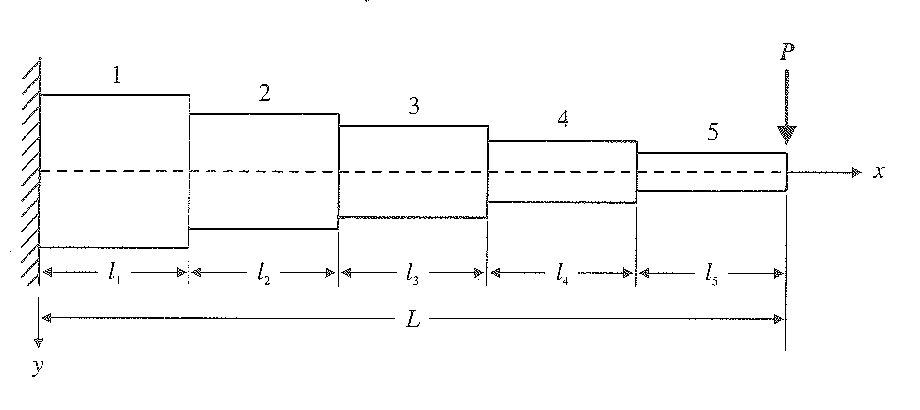
\includegraphics[width=1.0\textwidth]{beam.png}
    \caption{The cantilevered beam}
    \label{fig:beam}
\end{figure}

The design variables are the widths $b_i$ and heights $h_i$ of the segments. The number of segments $N$ can be chosen arbitrary. The total length of the beam is 500 cm, the lengths of the segments are $l_i=500/N$  cm. There are $N$ geometric constraints (the aspect ratios of each block (i.e. heights divided by widths) should not exceed 20) and $N$ constraints on the stress, calculated at the left end of each segment (stresses should not exceed  $\bar{\sigma}=14000\; N/cm^2$). There is also also a constraint on the displacement at the tip, which should not exceed 2.5 cm. The load is $P = 50 000\; N$, the Young's modulus is $E=2\cdot 10^7  N/cm^2$.

The deflection $y_i$ at the right hand of the $i$-th segment is given by the following recursive formulas:
\begin{displaymath}
  \begin{array}{c}
    y_0=y_0'=0, \\
    y_i'=\frac{P\cdot l_i}{E\cdot I_i}\Big[ L+\frac{l_i}{2}-\sum\limits_{j=1}^i l_j\Big]+y_{i-1}', \\
    y_i=\frac{P\cdot l_i^2}{2E\cdot I_i}\Big[L-\sum\limits_{j=1}^i l_j + \frac{2l_i}{3}\Big]+y_{i-1}'l_i+y_{i-1}.
  \end{array}
\end{displaymath}
The moment of inertia of a segment is $I_i=\frac{b_i h_i^3}{12}$ and the bending moment at the left end is $M_i=P[L+l_i- \sum_{j=1}^{i}  l_j ]$. The maximum bending stress in the segment $i$ is then given by the following formula:
\begin{displaymath}
  \sigma_i=\frac{M_i h_i}{2I_i}
\end{displaymath}

We are looking for a design with smallest volume $V = \sum_{i=1}^N b_i h_i l_i$. The widths $b_i$ vary from 1.0 to 10.0 cm and the heights $h_i$ from 5.0 to 100.0 cm. The optimization problem is formulated as follows:
\begin{displaymath}
  \begin{array}{c}
    \min\limits_{ b,  h}V( b,  h) \\
    s.t.\;1.0\le b_i \le 10.0, \\
    5.0 \le h_i \le 100.0, \\
    y_N\le 2/5, \\
    \sigma_i \le \bar{\sigma}=14000, \\
    \frac{h_i}{b_i}\le 20.
  \end{array}
\end{displaymath}

With $N=50$ segments (corresponding to 100 design variables) the SQP solution of this problem is $V = 63704.598\; cm^3$. The optimal values of design variables are given below (the first 50 entries are the widths and the last 50 entries are the heights of the segments):
\setcounter{MaxMatrixCols}{11}
\[
\begin{matrix}%[pos]{spalten}
			b=& \left[3.246, \right.& 3.224,& 3.202,& 3.179,& 3.156,& 3.133,& 3.109,& 3.085,& 3.061,& 3.036,  \\  
			  & 3.011,& 2.985,& 2.959,& 2.933,& 2.905,& 2.878,& 2.850,& 2.821,& 2.792,& 2.762, \\
			  & 2.731,& 2.700,& 2.668,& 2.635,& 2.602,& 2.567,& 2.532,& 2.495,& 2.458,& 2.419, \\  
			  & 2.379,& 2.338,& 2.295,& 2.250,& 2.204,& 2.156,& 2.105,& 2.052,& 1.996,& 1.936, \\  
			  & 1.873,& 1.805,& 1.732,& 1.651,& 1.562,& 1.462,& 1.345,& 1.196,& 1.023,& \left. 1.000\right] 	
\end{matrix}
\]
\[
\begin{matrix}
	h=& \left[64.919,\right.&64.480,&64.033,&63.581,&63.122,&62.656,&62.184,&61.703,&61.216,&60.720  \\
		& 60.216,&59.703,&59.182,&58.651,&58.110,&57.558,&56.996,&56.423,&55.837,&55.239  \\
		& 54.628,&54.003,&53.363,&52.707,&52.035,&51.344,&50.635,&49.906,&49.155,&48.381  \\
		& 47.582,&46.754,&45.897,&45.008,&44.082,&43.116,&42.105,&41.041,&39.919,&38.729  \\
		& 37.462,&36.102,&34.630,&33.020,&31.240,&29.241,&26.910,&23.919,&20.465,&\left.14.639 \right]
\end{matrix}
\]

MAM obtained the solution $V = 63935.360\; cm^3$, using 1500 function evaluations (as compared to almost 8000 evaluations used by SQP). The number of points in a trust region used to build approximations was 150. The optimal values of design variables obtained by MAM are given below:
\[
\begin{matrix}
	b=&	\left[3.238,\right.&3.204,&3.202,&3.170,&3.176,&3.128,&3.108,&3.089,&3.057,&3.003 \\  
		& 3.027,&2.986,&2.959,&2.952,&2.885,&2.855,&2.864,&2.847,&2.803,&2.762 \\  
		& 2.737,&2.722,&2.630,&2.645,&2.590,&2.558,&2.547,&2.480,&2.693,&2.391 \\ 
		& 2.368,&2.310,&2.307,&2.227,&2.176,&2.149,&2.106,&2.016,&2.007,&1.925 \\  
		& 1.864,&1.843,&1.758,&1.635,&1.582,&1.934,&1.332,&1.173,&1.026,&\left.2.419\right]
\end{matrix}
\]
\[
\begin{matrix}
	h=& \left[64.764,\right.&64.083,&64.036,&63.392,&63.518,&62.566,&62.153,&61.772,&61.149,& 60.054  \\
		& 60.534,&59.728,&59.182,&59.033,&57.695,&57.105,&57.274,&56.943,&56.057,&55.233  \\
		& 54.747,&54.433,&52.590,&52.902,&51.802,&51.150,&50.943,&49.597,&51.567,&47.811  \\
		& 47.373,&46.190,&46.140,&44.543,&43.525,&42.991,&42.119,&40.308,&40.141,&38.506  \\
		& 37.268,&36.839,&35.153,&32.702,&31.615,&28.304,&26.642,&23.447,&20.536,& \left.9.417\right]
\end{matrix}
\]

The solution obtained by MAM is very close to the reference solution obtained by SQP, except for the last design variable (the height of the last segment), which indicates that the problem is insensitive to this variable near the optimum, making it hard for the metamodels to capture this dependence. Both SQP and MAM solutions are, however, feasible and differ only slightly in the value of the objective function.

Next, let us compare the worktime of the sequential and parallel algorithms when solving the large scale problems. 
The dimensionality of the problem being solved $N$ was varied from 100 up to 1000 design variables that corresponds to 50 to 500 segments of the cantilevered beam. The number of points in a trust region used to build the approximations was $1.5 N$. 
Both algorithms was run on a single node of the cluster (the specifications of the node are listed below), the parallel algorithm employed all 16 processors cores available. Since the time of computing of the objective 
function and constraints in the test problem being solved was negligible, these ones were computed on the same node.

Table 1 reflects the worktime (in seconds) of the sequential algorithm and of the parallel one subject to the number of variables. In Table 2, the number of MAM iterations $I_{MAM}$ as well as the number of the function evaluations $F_{MAM}$ required for solving the problem are presented. For comparison, the number of the function value computations, which would be required to solve the initial (non-approximated) problem by SQP method $F_{SQP}$ is given also. In all conducted experiments, the objective function values in the sequential and parallel versions of the algorithm were the same (up to the accuracy of the computational error) and differed from the solution obtained by SQP negligibly. The reduction of the number of the function evaluations required to solve the problem using MAM as compared to the use of SQP was demonstrated 
visibly.

\begin{table}
	\caption{Time and speedup}
	\label{tab:1}
	\center
	\begin{tabular}{cccc}
		\hline\noalign{\smallskip}
		$N$ & $T_{MAM}$ & $T_{PMAM}$ & Speedup \\
		\hline\noalign{\smallskip}
		100 & 15.4 & 11.9 & 1.3  \\
		200 & 167 &  89 &  1.9 \\
		500 & 5151 &  1520 & 3.4  \\
		1000 & 67674 &  13771 & 4.9  \\
		\noalign{\smallskip}\hline
	\end{tabular}
\end{table}

\begin{table}
	\caption{Function evaluations}
	\label{tab:2}
	\center
	\begin{tabular}{cccc}
		\hline\noalign{\smallskip}
		$N$ & $I_{MAM}$  & $F_{MAM}$ & $F_{SQP}$ \\
		\hline\noalign{\smallskip}
		100 & 10 &  2201 & 9901 \\
		200 & 10 &  4402 & 28143 \\
		500 &  &   &  115734 \\
		1000 &  &   & 305308 \\
		\noalign{\smallskip}\hline
	\end{tabular}
\end{table}

Computational experiments were carried out on a high-performance cluster of Lobachevsky State University of Nizhny Novgorod. The cluster node included two Intel Sandy Bridge E5-2660 2.2 GHz CPUs and 64 Gb RAM. The CPU had 8 cores, i.e. a total of 16 physical cores were available in the node. MS Visual Studio 15 and Intel Fortran Compiler were used to implement the algorithm.

\section{Conclusions}

Recent developments in the Multipoint Approximation Method (MAM) made it capable of solving large scale industrial optimization problems. The fact that MAM solves the initial problem by using the approximations of the objective function and constraints is the primary distinctive feature of the method. Within the framework of the present study, the parallel version of MAM oriented onto the reduction of the worktime of the optimization algorithm (assuming that computing the values of the objective function and constraints has been parallelized already) has been developed. The performed experiments have demonstrated an acceptable speedup when solving the large scale problems employing 16 cores on a single cluster node. The performance was demonstrated on a benchmark example of structural 
optimization known as the scalable cantilevered beam. 

\begin{thebibliography}{10}

\bibitem{Toropov1989}
Toropov, V.:
\newblock Simulation approach to structural optimization.
\newblock Structural Optimization \textbf{1}, 37--46 (1989)

\bibitem{Toropov1992}
Toropov, V.:
\newblock Multipoint approximation method in optimization problems with expensive function values.
\newblock In: Sydow, A. (ed.) Proceedings of the 4th international symposium on Systems analysis and simulation, 
pp. 207--212, Elsevier,  (1992)

\bibitem{ToropovFilatov1993}
Toropov, V., Filatov, A., Polynkin, A.:
\newblock Multiparameter structural optimization using fem and multipoint explicit approximations.
\newblock Structural Optimization \textbf{6}, 7--14 (1993)

\bibitem{ShahparPolynkinToropov2008}
Shahpar, S., Polynkin, A., Toropov, V.:
\newblock Large scale optimization of transonic axial compressor rotor blades.
\newblock In:  49th AIAA/ASME/ASCE/AHS/ASC Structures, Structural Dynamics, and Materials Conference, AIAA, art. no. 2008-2056
 (2008)

\bibitem{PolynkinToropovShahpar2008}
Polynkin, A., Toropov, V., Shahpar, S.:
\newblock Design optimization of aircraft engine components.
\newblock In: Proc. of 7th ASMO UK / ISSMO Conf. on Engineering Design Optimization. Process and Product Improvement (2008)

\bibitem{PolynkinToropovShahpar2010}
Polynkin, A., Toropov, V., Shahpar, S.:
\newblock Multidisciplinary optimization of turbomachinery based on metamodel built by genetic programming.
\newblock In: 13th AIAA/ISSMO Multidisciplinary Analysis and Optimization Conference (2010)

\bibitem{KeulenToropovMarkine1996}
van Keulen, F., Toropov, V., Markine, V.:
\newblock Recent refinements in the multi-point approximation method in conjunction with adaptive mesh refinement.
\newblock In: McCarthy, J.M. (ed.) Proc. of ASME Design Engineering Technical Conferences and Computers
  in Engineering Conf., 1--12, ASME, Irvine CA (1996)

\bibitem{ToropovKeulenMarkine1996}
Toropov, V., van Keulen, F., Markine, V., de~Boer, H.:
\newblock Refinements in the multi-point approximation method to reduce the effects of noisy responses.
\newblock In: 6th AIAA/NASA/ISSMO Symp. on Multidisciplinary Analysis and Optimization,  pp. 941--951, AIAA (1996)

\bibitem{ToropovMarkineHolden1999}
Toropov, V., Markine, V., Holden, C.:
\newblock Use of mid-range approximations for optimization problems with functions of domain-dependent calculability.
\newblock In: 3rd ISSMO/UBCAD/UB/AIAA World Congress of Structural and Multidisciplinary Optimization (1999).

\bibitem{ToropovMarkine1996}
Toropov, V., Markine, V.:
\newblock The use of simplified numerical models as mid-range approximations.
\newblock In: 6th AIAA/NASA/ISSMO Symp. on Multidisciplinary Analysis and Optimization, pp. 952--958 (1996).

\bibitem{ToropovAlvarez1998}
Toropov, V., Alvarez, L.:
\newblock Creation of multipoint approximations using genetic programming.
\newblock In: Parmee, I.C. (ed.) Adaptive Computing in Design and Manufacture, 3rd Int. Conf.,
   pp. 21--24, PEDC, Dartington (1998)

\bibitem{PolynkinToropov2012}
Polynkin, A. Toropov, V.:
\newblock Mid-range metamodel assembly building based on linear regression for large scale optimization problems.
\newblock Structural and Multidisciplinary Optimization \textbf{45}(4), 515--527 (2012)

\bibitem{LancasterSalkauskas1981}
Lancaster, P. Salkauskas, K.:
\newblock Surfaces generated by moving least squares methods.
\newblock Mathematics of Computation \textbf{87}, 141--158 (1981)

\bibitem{Liszka1984}
Liszka, T.:
\newblock An interpolation method for an irregular net of nodes.
\newblock Int. J. Num. Meth. \textbf{20}, 1599--1612 (1984)

\bibitem{ChoiYounYang2001}
Choi, K., Youn, B., Yang, R.-J.:
\newblock Moving least squares method for reliability-based design optimization.
\newblock In: 4th World Congress of Structural and Multidisciplinary Optimization, Dalian, China (2001)

\bibitem{ToropovSchrammSahaiJones2005}
Toropov, V., Schramm, U., Sahai, A., Jones, R., Zeguer, T.:
\newblock Design optimization and stochastic analysis based on the moving least squares method.
\newblock In: Herskovits, J., Mazorche, S., Canelas, A. (eds.) 6th World Congress of Structural and Multidisciplinary Optimization, art. no. 9412 (2005)

\bibitem{PolynkinToropov2010}
Polynkin, A. Toropov, V.:
\newblock Recognition of design variable inter-dependencies using  cross-validated moving least-squares method.
\newblock In: Proceedings of the 51st AIAA/ASME/ASCE/AHS/ASC Structures, Structural Dynamics, and Materials Conference, AIAA, art. no. 2010-2985 (2010)

\bibitem{OllarToropovJones2014}
Ollar, J., Toropov, V., Jones. R.:
\newblock  Mid-range approximations in sub-spaces for MDO problems with disparate discipline attributes.
\newblock In: 15th AIAA/ISSMO Multidisciplinary Analysis and Optimization Conference, AIAA, art. no. 2014-2437 (2014)

\bibitem{KeulenToropov1997}
van Keulen, F. Toropov, V.:
\newblock New developments in structural optimization using adaptive mesh refinement and multi-point approximations.
\newblock Engineering Optimization \textbf{29}, 217--234 (1997)

\bibitem{PolynkinToropov2008}
Polynkin, A., Toropov, V., Shahpar, S.:
\newblock Adaptive and parallel capabilities in the multipoint approximation  method.
\newblock In: 12th AIAA/ISSMO Multidisciplinary Analysis and Optimization Conference, AIAA, art. no. 2008-5803 (2008)

\bibitem{Vanderpllaats2001}
Vanderplaats, G.:
\newblock Multidiscipline Design Optimization. 
\newblock Vanderplaats Research \& Development, Inc., Colorado Springs, (2001)

\end{thebibliography}



%\bibitem{Strongin2000}
%Strongin, R.G., Sergeyev, Y.D.: Global Optimization with Non-Convex Constraints. Sequential and Parallel Algorithms. Kluwer Academic Publishers, Dordrecht (2000); DOI: 10.1007/978-1-4615-4677-1
%
%\bibitem{Barkalov2002}
%Barkalov, K.A., Strongin, R.G.: A global optimization technique with an adaptive order of checking for constraints. Comput. Math. Math. Phys. 42(9), 1289--1300 (2002)
%
%\bibitem{Gergel2005}
%Gergel, V.P., Strongin, R.G.: Parallel computing for globally optimal decision making on cluster systems. Future Gener. Comput. Syst. 21(5), 673--678 (2005); DOI: 10.1016/j.future.2004.05.007
%
%\bibitem{Strongin2013}
%Sergeyev, Ya.D., Strongin, R.G., Lera, D.: Introduction to global optimization exploiting space-filling curves. Springer (2013);  DOI: 10.1007/978-1-4614-8042-6
%
%\bibitem{Barkalov2010}
%Barkalov, K., Ryabov, V., Sidorov, S.: Parallel Scalable Algorithms with Mixed Local-Global Strategy for Global Optimization Problems. In: Hsu, Ch., Malyshkin, V. (Eds.) MTPP 2010, LNCS, vol. 6083, pp. 232--240. Springer, Heidelberg (2010); DOI: 10.1007/978-3-642-14822-4$\_$26
%
%\bibitem{Barkalov2015}
%Barkalov, K., Gergel, V., Lebedev, I.: Use of Xeon Phi Coprocessor for Solving Global Optimization Problems. In: Malyshkin, V. (Ed.) PaCT 2015, LNCS, vol. 9251, pp. 307--318. Springer, Heidelberg (2015); DOI: 10.1007/978-3-319-21909-7$\_$31
%
%\bibitem{Barkalov2016}
%Barkalov, K., Gergel, V.: Parallel Global Optimization on GPU. J. Glob. Optim. 66(1), 3--20 (2016); DOI: 10.1007/s10898-016-0411-y
%
%\bibitem{Gergel2016}
%Barkalov, K., Gergel, V., Lebedev, I.: Solving Global Optimization Problems on GPU Cluster. In: Simos T.E. (Ed.) ICNAAM 2015, AIP Conference Proceedings, vol. 1738, art. no. 400006 (2016); DOI: 10.1063/1.4952194
%
%\bibitem{Gergel2015}
%Gergel, V., Sidorov, S.: A Two-Level Parallel Global Search Algorithm for Solution of Computationally Intensive Multiextremal Optimization Problems. In: Malyshkin, V. (Ed.) PaCT 2015, LNCS, vol. 9251, pp. 505--515. Springer, Heidelberg (2015); DOI: 10.1007/978-3-319-21909-7$\_$49
%

%\end{thebibliography}

\end{document}
